\subsection{Modelo conceptual}

Mostramos ahora nuestro modelo conceptual del sistema de la empresa. 

\begin{figure}[H]
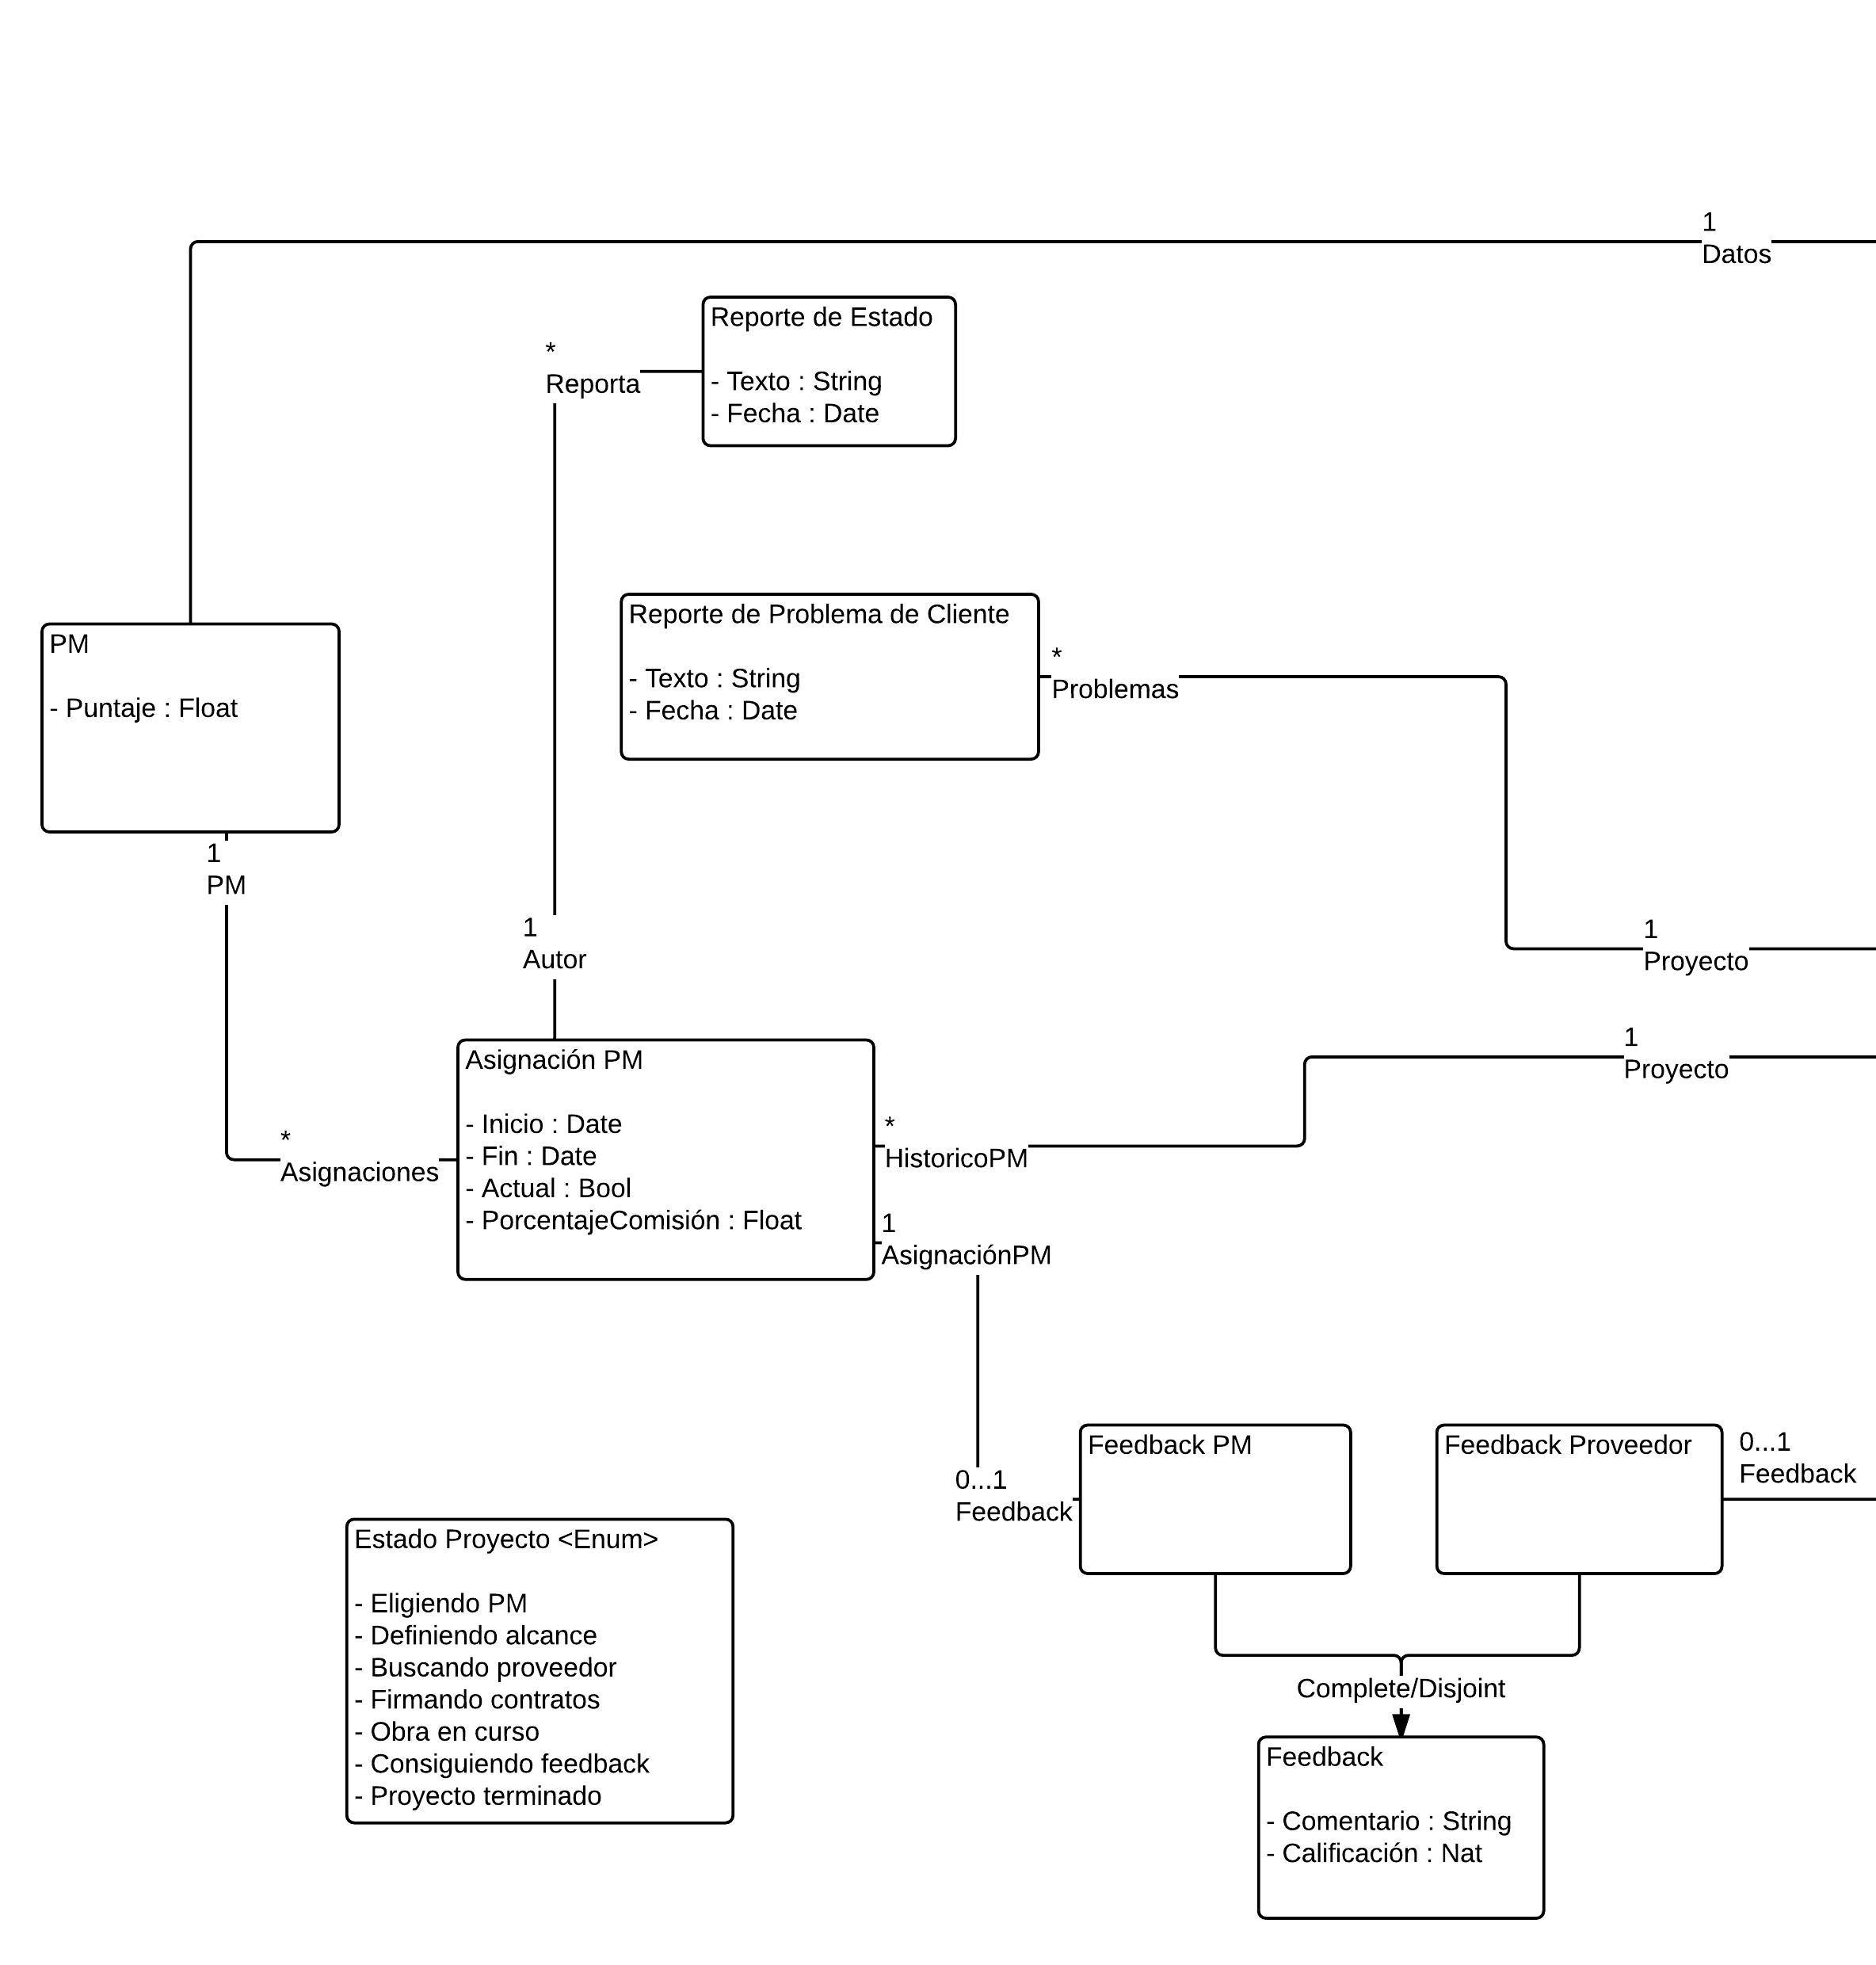
\includegraphics[width=\linewidth]{diag/nuevos/concept2.png}
\caption{Modelo conceptual (1)}
\label{concept1}
\end{figure}

\begin{figure}[H]
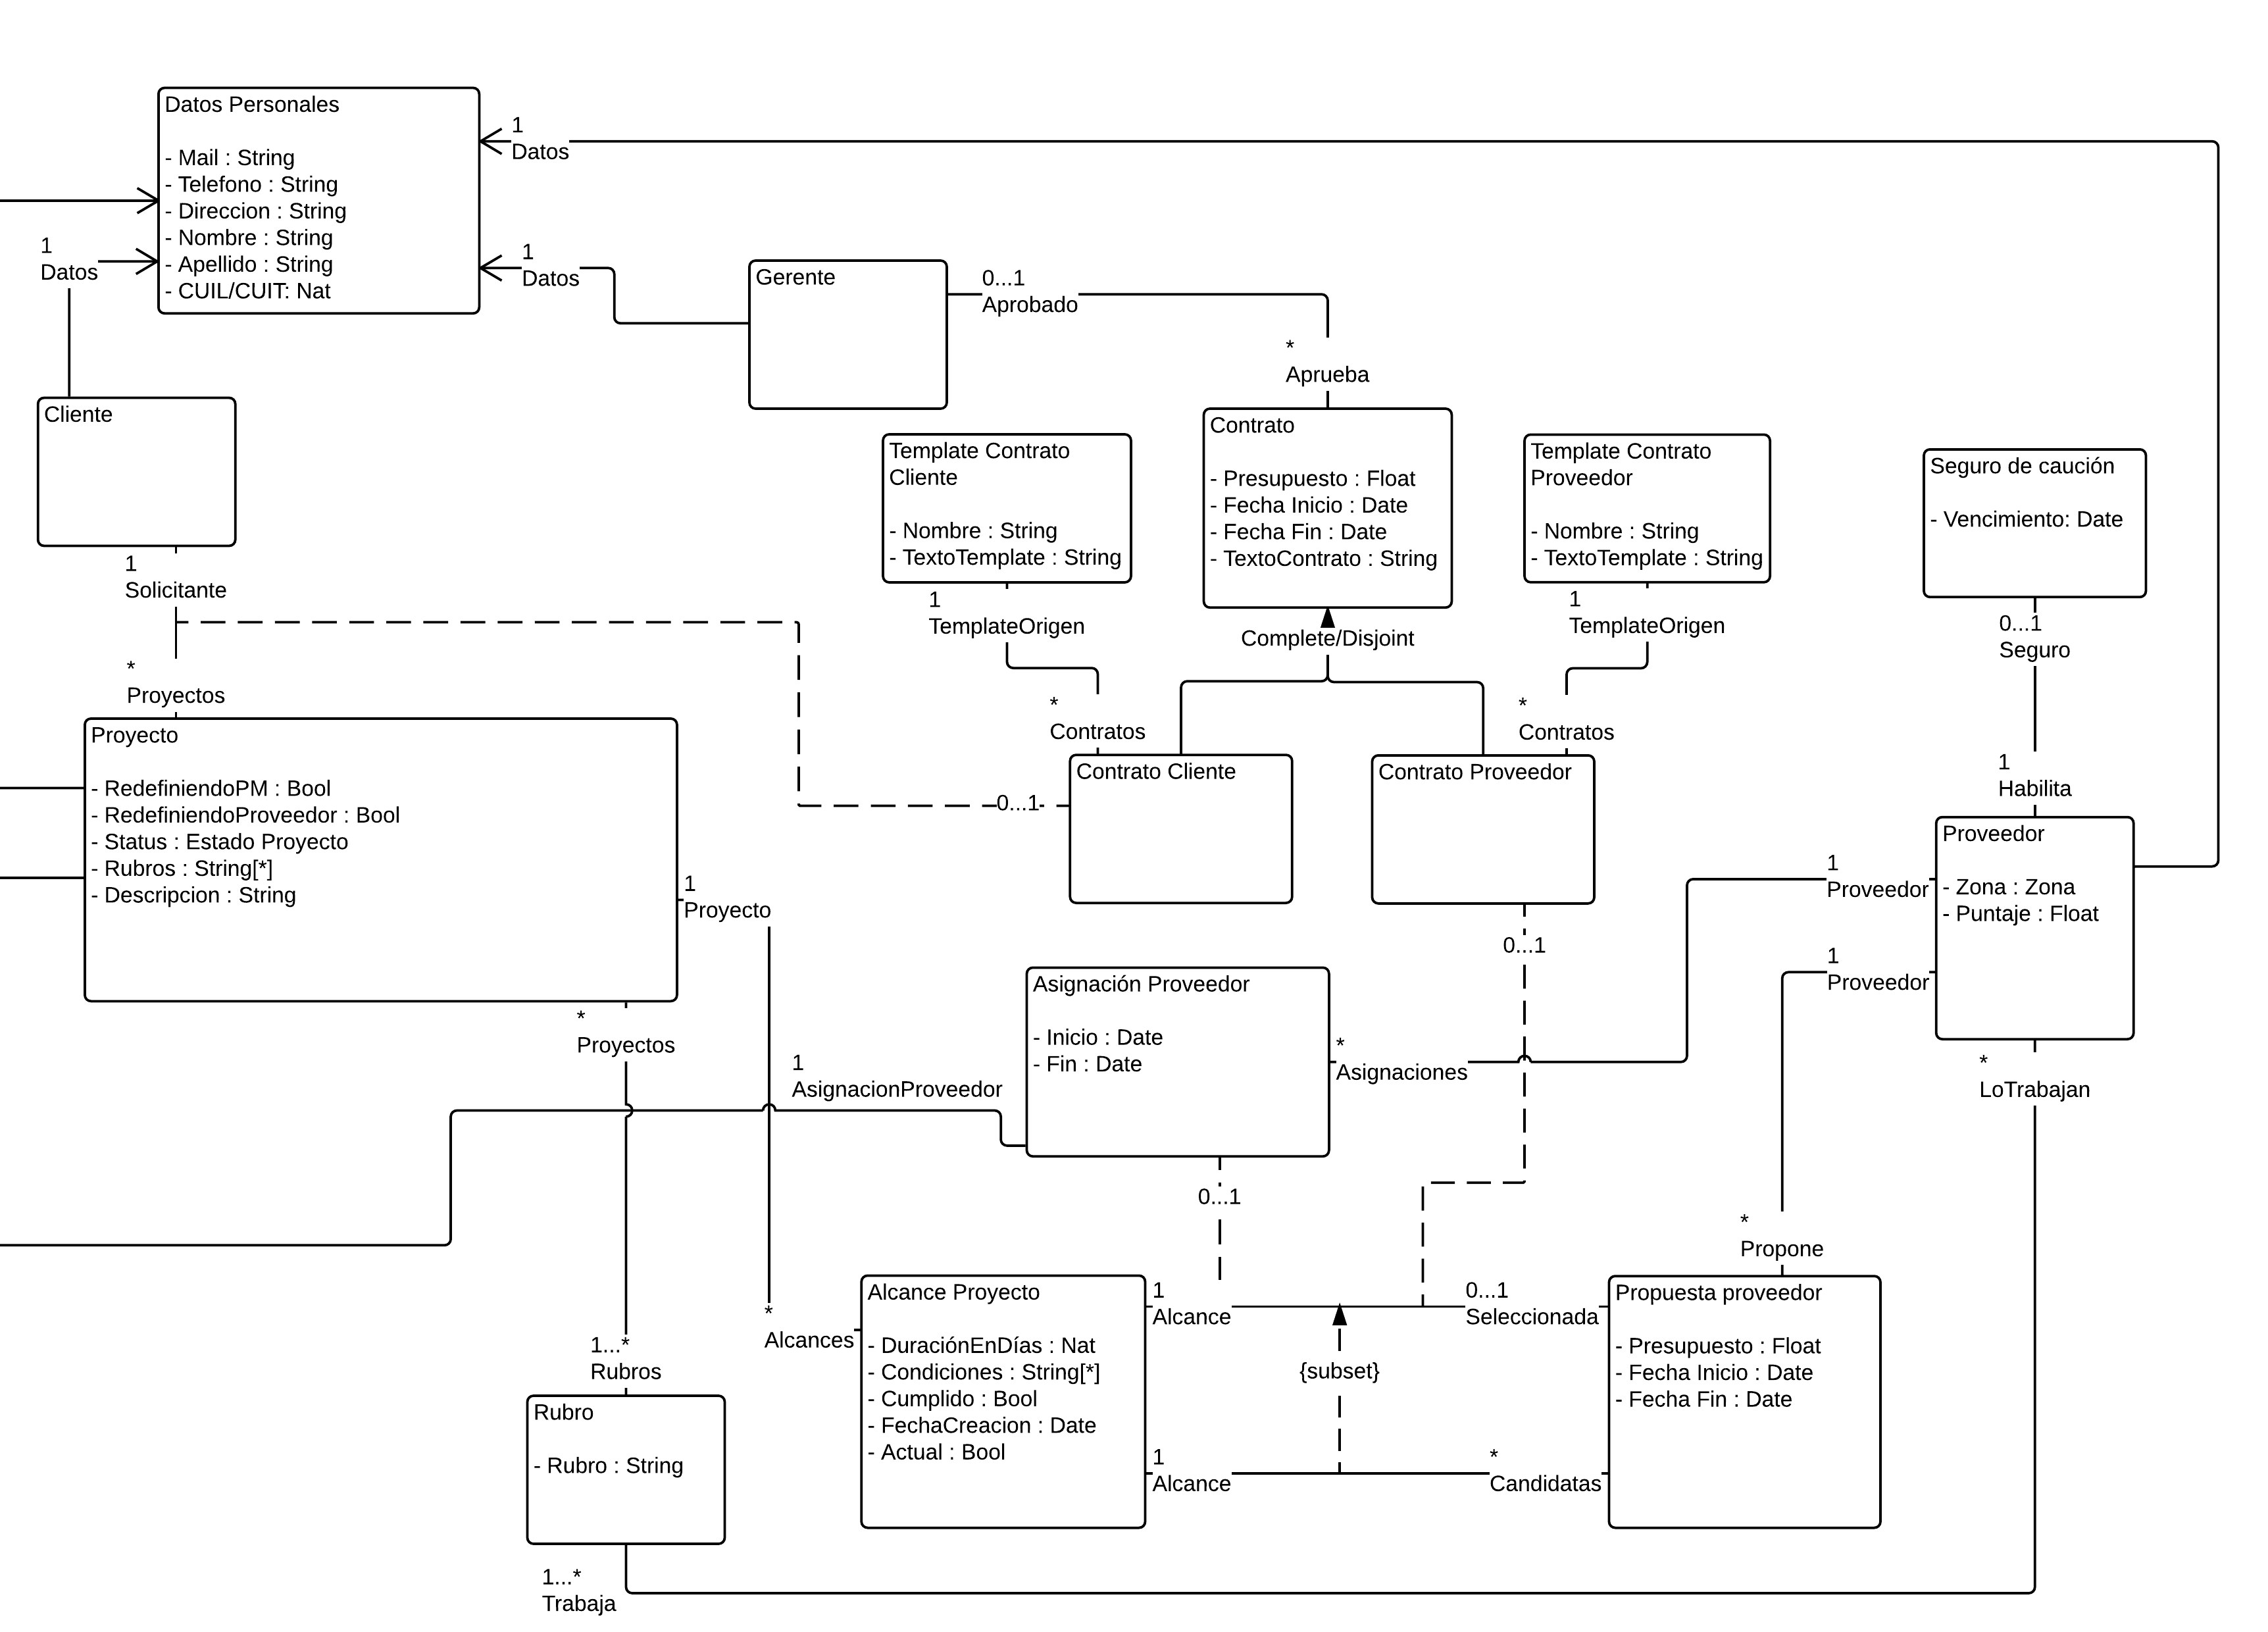
\includegraphics[width=\linewidth]{diag/nuevos/concept1.png}
\caption{Modelo conceptual (2)}
\label{concept2}
\end{figure}

En el mismo puede verse que la clase \textit{Proyecto} tiene un atributo \textit{Status} 
que es un enumerado, con los estados posibles. Estos estados no son exactamente los 
mismos que se enuncian en el FSM de flujo general del proyecto (figura \ref{fsm-proj}), sino más 
bien son un subconjunto que creemos apropiado. 

La idea es que ese \textit{Status} 
sea lo que los usuarios del sistema vean como estado del proyecto en la interfaz. 
Usamos ese atributo además para predicar distintas cosas por OCL, por ejemplo 
qué cosas debe tener cargadas un proyecto en determinada etapa. 

\subsubsection{Condiciones OCL}
\begin{itemize}
		\item	\textbf{Momentos en los cuales se puede redefinir el PM o proveedor de un proyecto:}
	
			\underline{Context: Proyecto}
			
			\begin{tabular}{ll}
				self.redefiniendoProveedor $\Rightarrow$	& BuscandoProveedor < self.Status $\leq$ ObraEnCurso	\\
				self.redefiniendoPM $\Rightarrow$			& EligiendoPM < self.Status $\leq$ ObraEnCurso			\\
			\end{tabular}

	\item \textbf{Estado del proyecto:}

			\underline{Context: Proyecto}
			
			\begin{tabular}{ll}
				\laterThan{EligiendoPM}				& \notEmpty{self.historicoPM} and	\\
													& ((self.redefiniendoPM) xor \\
													& (self.historicoPM\applyParam{exists}{pm$|$pm.Actual}))	\\
				
				and \laterThan{DefiniendoAlcance}	& \notEmpty{self.Alcances} \\
				
				and \laterThan{BuscandoProveedor}	& self.Alcances\applyParam{select}{a$|$a.Actual}.Seleccionada\notEmpty{}	\\
				
				and \laterThan{FirmandoContratos}	& \notEmpty{contratoCliente(self, self.Solicitante)} and	\\
													& (self.redefiniendoProveedor xor							\\
													& self.Alcances\applyParam{select}{a$|$a.Actual}.ContratoProveedor	\\
													& \notEmpty{})	\\
				
				and \laterThan{ConsiguiendoFeedback}	& self.HistoricoPM\applyParam{forAll}{a$|$
				a.\notEmpty{Feedback}} and	\\
														& self.Alcances\applyParam{collect}{AsignacionProveedor} \\
														& \applyParam{forAll}{a$|$a.Feedback\notEmpty{}} \\
			\end{tabular}
			
	\item \textbf{Seguro de caución al día para proyectos actuales:}
	
			\underline{Context: Alcance Proyecto}
			
			self.Actual $\Rightarrow$ (\notEmpty{self.Seleccionada.Proveedor.Seguro} \\
			and self.Seleccionada.Proveedor.Seguro.Vencimiento	\\
			$\geq$ self.ContratoProveedor.FechaFin)	\\
			
			%(self.Actual and self.Proyecto.Status $\in$ [BuscandoProveedor, obraEnCurso]	\\
			%and \notEmpty{self.PropuestaProveedor.contratoProveedor}) 		\\
			%$\Rightarrow$ (\notEmpty{self.Proveedor.Seguro} and self.Proveedor.Seguro.Vencimiento	\\
			%> self.PropuestaProveedor.contratoProveedor.FechaFin)	\\
			
	\item \textbf{Los puntajes de los agentes se corresponden con los puntajes seg\'un proyectos:}
			
			\underline{Context: PM}
			
			self.puntaje ==	self.Asignaciones\applyParam{collect}{FeedbackPM}\applyParam{collect}{Calificacion}\apply{average}
			\footnote{Consideramos que average de vacío da 0.}
			
			\underline{Context: Proveedor}
			
			self.puntaje ==	self.Asignaciones\applyParam{collect}{FeedbackProv}\applyParam{collect}{Calificacion}\apply{average}
			\footnote{Idem nota anterior}
			
	
	\item \textbf{Las asignaciones no se pisan en tiempo}
	
			\underline{Context: Proyecto}
			
			self.Alcances\applyParam{collect}{AsignacionProveedor}\applyParam{forAll}{a1 $\neq$ a2$\|$a1.Inicio > a2.Fin or a2.Inicio > a1.Fin}
			
			self.HistoricoPM\applyParam{forAll}{a1 $\neq$ a2$\|$a1.Inicio > a2.Fin or a2.Inicio > a1.Fin}
	
	\item \textbf{Hay a lo sumo un alcance actual y una asignación de PM actual}
	
			\underline{Context: Proyecto}
			
			self.Alcances\applyParam{select}{a$\|$a.Actual}\apply{count} $\leq$ 1
			
			self.HistoricoPM\applyParam{select}{a$\|$a.Actual}\apply{count} $\leq$ 1
			
			self.Status > ObraEnCurso $\Rightarrow$ self.Alcances\applyParam{select}{a$\|$a.Actual}\apply{count} = 0
			
	\item \textbf{Ciclo Proveedor - Asignaci\'on - Propuesta}
	
			\underline{Context: Asignación Proveedor}
			
			self.Proveedor == self.Seleccionada.Proveedor
	
	\item \textbf{Fechas de fin luego de fechas de inicio}
			
			\underline{Context: Asignación PM}
			
			self.FechaInicio < self.FechaFin
			
			\underline{Context: Contrato}
			
			self.FechaInicio < self.FechaFin
			
			\underline{Context: Asignación Proveedor}
			
			self.FechaInicio < self.FechaFin
			
			\underline{Context: Propuesta Proveedor}
			
			self.FechaInicio < self.FechaFin			
	
	\item \textbf{Definiciones de alcance actual}
	
			\underline{Context: Proyecto}
			
			(self.Alcances\applyParam{select}{a$|$a.Actual}\apply{count}<=1) and
			
			((self.Status > DefiniendoAlcance) and !self.RedefiniendoProveedor $\Rightarrow$
			
			(self.Alcances\applyParam{select}{a$|$a.Actual}\apply{count}==1))
			
	%\item \textbf{Los estados del proyecto pero para el otro lado?}
	
\end{itemize}
